\documentclass[11pt]{article}

\usepackage[margin=1in]{geometry}
\usepackage[T1]{fontenc}
\usepackage{lmodern}
\usepackage{microtype}
\usepackage{amsmath,amssymb}
\usepackage{booktabs}
\usepackage{threeparttable}
\usepackage{graphicx}
\usepackage{setspace}
\usepackage[round,authoryear]{natbib}
\usepackage[hidelinks]{hyperref}
\usepackage{caption}
\captionsetup{font=small,labelfont=bf}

\onehalfspacing
\newcommand{\dmse}{\Delta\mathrm{MSE}}

\title{Does Federal Reserve Communication Improve Policy-Rate Forecasts?\\[4pt]
\large Evidence from Look-Ahead-Controlled, Real-Time Walk-Forward Tests}
\author{[Author Name]\thanks{[Affiliation]. Working paper prepared for discussion with my supervisor. Code, result
files and the audit trail are in the project repository. All results labelled \emph{exploratory} were added after
earlier results had been seen; every change to the pre-registered plans is dated in \texttt{DEVIATIONS.md}.}}
\date{Draft of 13 October 2026}

\begin{document}
\maketitle

\begin{abstract}
\noindent
We ask whether the hawkish--dovish stance of Federal Reserve documents improves out-of-sample forecasts of the
federal funds rate beyond macroeconomic statistics and market prices. Stance is measured with two readers: a
chronologically consistent ChronoBERT classifier, retrained each year on earlier labels only, and sentence labels
from the large language model Claude Haiku. We forecast the monthly average effective rate (308 test months) and the
decision at each FOMC meeting (212 meetings) from 2001 to 2026 in expanding-window walk-forward tests, with ridge
regression, a penalised ordered logit, and LSTM, GRU and Temporal Fusion Transformer networks. Adding text lowers
squared error in most comparisons, but few gains survive testing. On a corrected monthly information cutoff, text
lowers the root mean squared error of a statistics-only ridge model from 0.192 to 0.168 percentage points
(one-sided Diebold--Mariano--HLN $p=0.103$), and 78\% of that gain comes from June 2020. Of six network comparisons
per task, only an LSTM reading Haiku stance on meeting decisions survives Holm adjustment (adjusted $p=0.020$); its
gain is not statistically established with strictly real-time inputs, and Haiku's training data cover the whole
test period. Once market prices are in the model, text changes monthly RMSE by less than 0.002 percentage points.
Fed communication features improved forecasts in some specifications, but the evidence does not yet establish a
consistent and reliable incremental benefit.

\medskip
\noindent\textbf{Keywords:} central bank communication; monetary policy; text as data; large language models;
look-ahead bias; forecast evaluation.\quad \textbf{JEL:} E52, E58, C53.
\end{abstract}

\newpage

%======================================================================
\section{Introduction}
%======================================================================

The Federal Reserve communicates constantly. Post-meeting statements, minutes, press conferences and speeches
are intended to shape expectations of the policy path, and asset prices respond to them
\citep{gss2005,hansen2016}. If this communication carries information about future decisions that is not already
in data and prices, a forecaster who reads it should outperform one who does not. This paper tests that
proposition under conditions designed to make a false positive difficult.

The question is deliberately narrow. Does the hawkish--dovish tone of Fed documents improve \emph{out-of-sample}
forecasts of the federal funds rate, \emph{beyond} macroeconomic statistics and market prices that were available
at the same moment? We study two tasks over 2001--2026: the monthly average effective federal funds rate and the
target rate set at each meeting of the Federal Open Market Committee (FOMC).

Recent work reports that neural networks and large language models (LLMs) forecast the policy rate well
\citep{chanlau2025}. Two problems make such results hard to interpret. First, LLMs trained on recent text may have
read about the very decisions they are asked to forecast \citep{lopezlira2025,sarkar2024,crane2025}. Second,
macroeconomic data are revised, and back-tests that use today's vintages give models information that forecasters
did not have \citep{croushore2001}. A text gain measured without controlling for both can reflect hindsight
rather than skill.

Our design addresses these problems in three ways.
\begin{enumerate}
  \item \textbf{A chronologically consistent reader.} Our primary text reader is ChronoBERT \citep{he2025}, which
        releases one model per year trained only on text up to that year. We fine-tune each year's classifier only
        on labelled sentences from documents dated before that year. A second reader, Claude Haiku, is used for
        comparison, and its memory of the test period is measured directly.
  \item \textbf{Real-time inputs.} Statistics are taken from ALFRED vintages released before each forecast cutoff.
        Results are reported separately for mixed-vintage, partially real-time and strictly real-time input sets.
  \item \textbf{Pre-specification and controls.} Hypotheses, tests and multiple-testing families were fixed
        before the main results; later changes are dated and labelled. Every text model is paired with a placebo
        in which the text features are permuted or shifted.
\end{enumerate}

The paper makes three contributions. It provides a pre-specified, look-ahead-controlled estimate of what Fed text
adds to policy-rate forecasts across linear models and three neural architectures. It compares a domain-trained,
time-consistent classifier with a general-purpose LLM on identical documents and protocol. And it documents how
fragile a headline gain can be: to a single month, to the information cutoff, and to the composition of the
multiple-testing family. An internal audit corrected two errors in our own earlier reporting, and the corrected
numbers are used throughout.

The answer is modest. Text lowers forecast error more often than it raises it, and one network comparison survives
correction. But the monthly gain rests largely on one month at the zero lower bound, the surviving meeting gain is
not established with strictly real-time inputs and comes from the reader that has seen the test period, and market
prices leave text almost nothing to add.

Section~\ref{sec:lit} reviews related work. Section~\ref{sec:data} describes the data and
Section~\ref{sec:methods} the methods. Section~\ref{sec:results} presents the results and
Section~\ref{sec:robust} the robustness analysis. Section~\ref{sec:disc} discusses limitations and
Section~\ref{sec:concl} concludes.

%======================================================================
\section{Related literature}\label{sec:lit}
%======================================================================

\paragraph{Central bank communication and asset prices.}
\citet{gss2005} show that FOMC statements move asset prices through a ``path'' factor distinct from the
surprise in the target rate, and \citet{gss2007} show that market-based measures are strong predictors of the
policy path. \citet{lucca2009} and \citet{hansen2016} measure the content of Fed language directly. These studies
mostly ask whether words move prices on announcement days. We ask a different question: whether words help
forecast later decisions once prices are already known.

\paragraph{Text-based stance measures.}
Dictionary approaches \citep{loughran2011} have given way to supervised classifiers trained on hand-labelled
sentences. Trillion Dollar Words \citep{shah2023} and the World Central Banks dataset \citep{shah2025} provide
hawkish, dovish and neutral labels for Fed sentences, and we use both. Newspaper sentiment \citep{shapiro2022},
geopolitical risk \citep{caldara2022} and economic policy uncertainty \citep{baker2016} provide further
text-derived indicators.

\paragraph{Machine-learning forecasts of the policy rate.}
\citet{chanlau2025} report accurate federal funds rate forecasts from LSTM and GRU networks and from an LLM.
We attempted to replicate their LSTM and GRU results and did not succeed: on their January 2016 to April 2025
window, our real-time versions reach RMSE 0.415 and 0.647 percentage points against 0.238 and 0.271 published,
while a no-change forecast scores 0.192.

\paragraph{Look-ahead bias in language models.}
\citet{lopezlira2025} show that GPT-4o recalls economic series before its training cutoff and that masking and
instructions do not remove this; \citet{sarkar2024} and \citet{crane2025} document related forms of look-ahead.
The most common remedy is a chronologically consistent model \citep{he2025}. \citet{glasserman2023} and
\citet{engelberg2025} propose masking diagnostics, and \citet{eliseev2026} propose fake-date tests.

\paragraph{Forecast evaluation.}
We compare nested forecasts with the test of \citet{diebold1995} and the small-sample correction of
\citet{hln1997}, \citet{newey1987} standard errors, \citet{mcnemar1947} tests for decision accuracy and
\citet{holm1979} adjustment within pre-registered families. The random walk is the standard benchmark
\citep{meese1983}.

%======================================================================
\section{Data}\label{sec:data}
%======================================================================

The sample runs from January 1994 to September 2026. Rows before 2001 are used for training only, and forecasts
are evaluated from January 2001.

\subsection{Targets}

\begin{table}[ht]\centering\small
\caption{Forecasting tasks}\label{tab:tasks}
\begin{tabular}{p{2.6cm}p{6.6cm}p{5.2cm}}
\toprule
Task & Target & Test sample \\ \midrule
T1, monthly & Monthly average effective federal funds rate (FRED \texttt{FEDFUNDS}); models forecast the change
from the last observed month & 308 months, Jan 2001--Sep 2026 (Jan 2004 dropped for missing data) \\
T2, per meeting & Target set at each FOMC meeting (midpoint of the range) and its class: cut, hold or hike, with a
$\pm 0.125$ percentage-point band & 212 meetings incl.\ 6 unscheduled; the network study uses the 206 scheduled
meetings \\
\bottomrule
\end{tabular}
\end{table}

\subsection{Inputs}

Table~\ref{tab:blocks} lists the input blocks. Statistics (S) follow \citet{chanlau2025} without the commercial
property index, which has no free equivalent. Market variables (M) are FRED daily series as of the cutoff.

\begin{table}[ht]\centering\small
\caption{Input blocks}\label{tab:blocks}
\begin{tabular}{p{2.8cm}p{8.6cm}p{3.2cm}}
\toprule
Block & Content & Source \\ \midrule
S, statistics (16) & Lagged policy rate; M2 (monthly and 12-month change); PCE and core PCE inflation;
payroll change; average weekly earnings; nominal GDP growth; U-6 (monthly and 12-month change); PPI; CPI and core
CPI; FHFA house prices; 10y--2y and 1y--6m yield slopes & FRED/ALFRED vintages \\
M, markets (8) & 3-month bill and 6-month, 1-year and 2-year yield spreads to the target; target level;
zero-lower-bound flag; VIX; WTI oil & FRED daily \\
N, news (6) & Fed stance and its change; Beige Book net tone; newspaper sentiment; geopolitical risk; policy
uncertainty & Section~\ref{sec:stance} \\
Fed text & 2,840 documents: 240 statements, 263 minutes, 94 press-conference transcripts, 262 Beige Books, 1,981
Board speeches & federalreserve.gov \\
Labels & Hawkish, dovish and neutral sentences from Trillion Dollar Words and the Fed subset of World Central Banks
& \citet{shah2023,shah2025} \\
\bottomrule
\end{tabular}
\end{table}

\subsection{Information cutoffs and data vintages}\label{sec:vintage}

Each statistic is the latest ALFRED vintage released strictly before the forecast cutoff. Where ALFRED has no
vintage, the earliest available vintage with a conservative release lag is used; those values include later
revisions. First vintages begin in 2011 for average weekly earnings and U-6 and in 2012 for house prices. As a
result, 136 of 308 monthly and 96 of 212 meeting test rows (44--45\%) use at least one revised value. We therefore
report three vintage treatments:
\begin{itemize}
  \item \textbf{Mixed vintage}: the full input set, with disclosed fallback values;
  \item \textbf{Partial}: the four fallback columns removed from the inputs, although fallback values remain in
        pre-2001 training rows;
  \item \textbf{Strict real-time}: only the eight series with complete vintages (policy-rate lag, M2 monthly and
        yearly change, payrolls, nominal GDP, CPI and the two yield slopes), plus M for meetings. No fallback value
        enters tuning, training or prediction.
\end{itemize}

\paragraph{Monthly cutoff correction.}
The original monthly panel dated each forecast at the first calendar day of month $t$, when FEDFUNDS$(t-1)$ is
not guaranteed to have been published. A corrected panel places the cutoff at 00:00 New York time at the start of
the second US business day of month $t$. The network study used the corrected panel from the start; the linear
monthly models were rerun on it after the audit (Section~\ref{sec:cutoff}).

\paragraph{Label dating.}
The published year field of Trillion Dollar Words does not always match the document date, which would leak
future labels into training. Each label is dated by the earliest corpus document that contains it; the 10.7\% of
Trillion Dollar Words and 1.7\% of World Central Banks sentences that match no document are dropped.

%======================================================================
\section{Methods}\label{sec:methods}
%======================================================================

\subsection{Measuring stance}\label{sec:stance}

\paragraph{ChronoBERT (C).}
For each classifier year $y\geq 2000$ we start from the ChronoBERT backbone trained on text published up to
31 December of year $y-1$ (2025 and 2026 use the 2024 vintage). A linear layer on the mean-pooled last hidden state
classifies each sentence as dovish, hawkish or neutral. It is trained only on labels whose source document is dated
before 1 January of year $y$, with AdamW (learning rate $2\times10^{-5}$, weight decay 0.01), 3 epochs, batch size
16, at most 256 tokens, and three seeds whose probabilities are averaged. Documents of year $y$ are scored only by
the classifier of year $y$. Held-out sentence accuracy rises from 0.56 in 2000 to 0.70 in 2025 (mean 0.644), against
0.42--0.56 for always predicting the most common class.

\paragraph{Claude Haiku (H).}
The pinned model snapshot \texttt{claude-haiku-5-5} labels 343,742 sentences from 2,578 statements, minutes,
press conferences and speeches. Sentences are masked, shuffled and sent 25 per request; 343,717 receive a label,
of which 8.5\% are hawkish and 12.4\% dovish. On a pilot sample Haiku agrees with the human labels on 67.3\% of
sentences. Its training data extend to June 2026, so it has seen the entire test window
(Section~\ref{sec:disc}).

\paragraph{Aggregation.}
For sentence $i$ the stance score is
\begin{equation}
  s_i = \begin{cases}
    \hat P_i(\text{hawkish}) - \hat P_i(\text{dovish}) & \text{ChronoBERT},\\
    +1,\ 0,\ -1 \text{ for hawkish, neutral, dovish} & \text{Haiku}.
  \end{cases}
\end{equation}
A document's stance is the mean of $s_i$ over its sentences of 30--1,000 characters. For each forecast row, the
stance is the mean of three group means---statements with press conferences, minutes, and speeches---computed over
documents released since the previous cutoff and carried forward when no document appears:
\begin{equation}
  \text{stance}_t = \tfrac{1}{|G_t|}\sum_{g\in G_t}\ \tfrac{1}{|D_{g,t}|}\sum_{d\in D_{g,t}} \bar s_d,
\end{equation}
where $G_t$ is the set of non-empty groups. The text block used in the network and Study~4 ordered-logit models
($C$ or $H$) is $\text{stance}_t$ and its change from the previous row. Block N in the Plan~1 linear models adds
Beige Book tone (Loughran--McDonald net tone), newspaper sentiment, and the logs of the geopolitical-risk and
policy-uncertainty indices.

\subsection{Forecasting models}

\paragraph{Benchmarks.}
The no-change forecast sets next month's rate to the last observed value and holds the target at each meeting.
An inertial Taylor rule \citep{taylor1993} regresses the rate on its lag, real-time core PCE inflation and
real-time U-3 unemployment.

\paragraph{Ridge regression (T1).}
The monthly model forecasts the change in the rate,
\begin{equation}
  \hat\beta = \arg\min_\beta \sum_{\tau\le t-2} \bigl(\Delta r_\tau - x_\tau'\beta\bigr)^2 + \lambda\lVert\beta\rVert_2^2,
  \qquad \hat r_t = r_{t-1} + x_t'\hat\beta,
\end{equation}
with $\lambda$ chosen from seven log-spaced values between 0.1 and 1,000.

\paragraph{Penalised ordered logit (T2).}
For the decision class $y_m\in\{\text{cut}<\text{hold}<\text{hike}\}$ at meeting $m$,
\begin{equation}
  \Pr(y_m\le j\mid x_m) = \Lambda(\kappa_j - x_m'\beta),\qquad j\in\{\text{cut},\text{hold}\},
\end{equation}
estimated with an L2 penalty on $\beta$ chosen from $\{0.01,0.03,0.1,0.3,1,3\}$. The class forecast is the most
probable class; the rate forecast is the standing target plus the probability-weighted mean move, with mean move
sizes per class taken from the training window.

\paragraph{Neural networks.}
We use an LSTM \citep{hochreiter1997}, a GRU \citep{cho2014} and a single-horizon network inspired by the Temporal
Fusion Transformer \citep[TFT;][]{lim2021}, comprising variable-selection networks, an LSTM encoder, gated skip
connections and interpretable multi-head attention. All networks forecast the change in the rate, are trained with
Adam on mean squared error, and average eight seeds. Hyperparameters are tuned inside each training window on five
identical validation folds per candidate, scored in rate units, and the networks are refit every 12 months or eight
meetings (the version~2 protocol, Section~\ref{sec:prereg}).

\subsection{Walk-forward design}

Every model is re-estimated on an expanding window and forecasts only rows it has never seen. The forecast for
month $t$ is trained on rows up to $t-2$, because the outcome for month $t-1$ is not known at the cutoff. Meeting
forecasts are trained on earlier meetings only. Standardisation, penalty selection, hyperparameter search and early
stopping use training rows only; penalties are chosen by five-fold expanding-window cross-validation.

\subsection{Controls}

The \emph{placebo} replaces the text features with uninformative versions: permuted across rows inside each
training window in the linear models, and circularly shifted by half the panel in the networks. A placebo gain
would signal that text helps through spurious structure. The \emph{shuffled-label} control permutes training
targets, to check that the pipeline cannot forecast without signal.

\subsection{Tests}

Let $e_{b,t}$ and $e_{x,t}$ be the forecast errors of the base model and the model with text, and define the loss
differential
\begin{equation}
  d_t = e_{b,t}^2 - e_{x,t}^2,\qquad \dmse = \bar d = \tfrac1n\textstyle\sum_t d_t ,
\end{equation}
so that $\dmse>0$ favours text. The registered test for the linear models is the one-sided Diebold--Mariano
statistic with the Harvey--Leybourne--Newbold correction,
\begin{equation}
  \text{DM-HLN} = \sqrt{\frac{n+1-2h+h(h-1)/n}{n}}\;\frac{\bar d}{\sqrt{\hat V(\bar d)}}\ \sim\ t_{n-1},
\end{equation}
with horizon $h=1$. The network test is a one-sided $t$-test on $\bar d$ with \citet{newey1987} standard errors,
using lags equal to the refit interval (12 months or 8 meetings). Effect sizes are reported as $\dmse$ with a 90\%
paired moving-block bootstrap interval (block length equal to the refit interval, 10,000 draws, seed 0). Decision
accuracy is compared with McNemar's exact test on the meetings one model fixes and the other breaks.

Within a family of $m$ tests with ordered raw $p$-values $p_{(1)}\le\dots\le p_{(m)}$, Holm-adjusted values are
\begin{equation}
  \tilde p_{(k)} = \max_{j\le k}\ \min\{1,\ (m-j+1)\,p_{(j)}\}.
\end{equation}

\subsection{Pre-specification and analysis roles}\label{sec:prereg}

Table~\ref{tab:holm} lists the testing families. Plan~1 (linear models) and Plan~2 (first neural models) were
registered with git tags before results. The version~2 network protocol was written on 13 October 2026, after
the version~1 network results had been seen and an external review had found defects; it is a dated amendment,
not a pre-registration, and version~1 results are superseded. Analyses added after results are labelled
exploratory.

\begin{table}[ht]\centering\small
\begin{threeparttable}
\caption{Testing families and outcomes}\label{tab:holm}
\begin{tabular}{p{4.0cm}p{6.2cm}cp{3.4cm}}
\toprule
Study & Family & Size & Survivors at 0.05 \\ \midrule
Plan 1, H1 (registered) & Conjunctive: monthly DM-HLN, meeting DM-HLN and McNemar must all pass & 3 & None \\
Plans 1--2, H2 (registered) & Holm across the H2 tests that ran (H2a 10, H2c 2, H2d 3) & 15 & 1, H2c (not a text increment)\tnote{a} \\
Study 4, ordered logit & Single primary & 1 & None ($p=0.144$) \\
Study 4 networks, T2 (amendment) & Holm, 3 architectures $\times$ 2 readers & 6 & LSTM + Haiku (0.020) \\
Study 4 networks, T1 (amendment) & Holm, 3 architectures $\times$ 2 readers & 6 & None (min.\ 0.156) \\
Study 5, three meetings ahead & Single primary; Holm across 4 secondaries & 1+4 & None \\
\bottomrule
\end{tabular}
\begin{tablenotes}\footnotesize
\item[a] H2c compares the meeting model with text against the random walk ($p=0.0044$); it does not measure what
text adds over a model without text.
\end{tablenotes}
\end{threeparttable}
\end{table}

%======================================================================
\section{Results}\label{sec:results}
%======================================================================

Throughout, RMSE is in percentage points and $\dmse$ in squared percentage points, with positive values favouring
text. Figure~\ref{fig:rates} shows the monthly forecasts against the actual rate.

\begin{figure}[ht]\centering
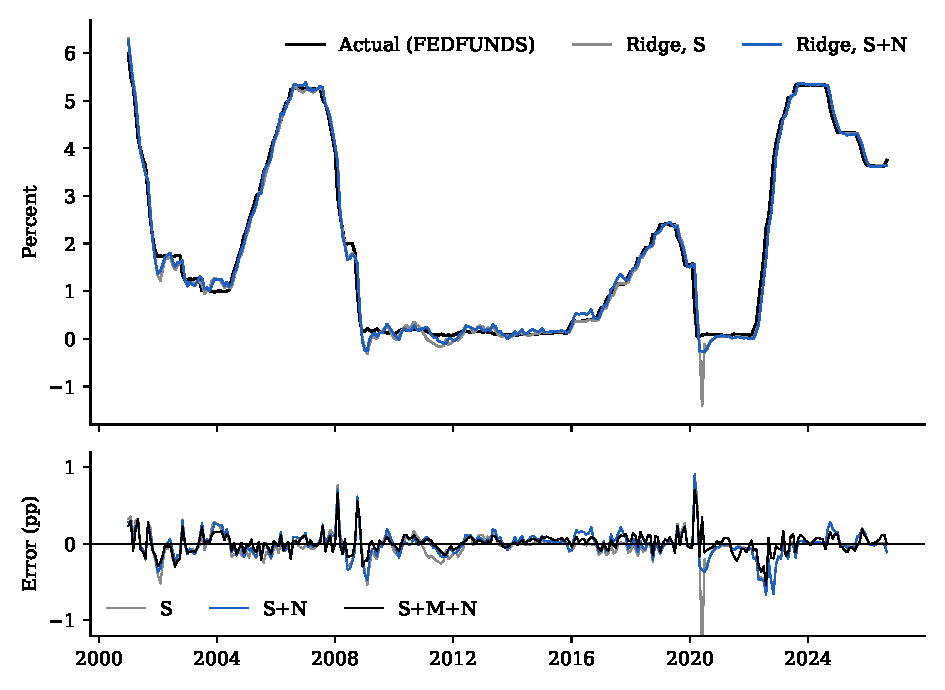
\includegraphics[width=\textwidth]{figures/fig_rates.pdf}
\caption{Monthly federal funds rate and walk-forward ridge forecasts on the corrected cutoff, January 2001 to
September 2026. Lower panel: forecast errors (forecast minus actual) for the statistics-only (S), statistics plus
news (S+N) and full (S+M+N) models.}\label{fig:rates}
\end{figure}

\subsection{Linear models}

No registered linear hypothesis is supported (Table~\ref{tab:linear}). Adding text to statistics gives the
largest relative gain in the monthly task, a 13\% lower RMSE, but its 90\% interval includes zero and the
registered test gives $p=0.103$. Once market prices are included, text changes monthly RMSE by 0.0017 and
meeting RMSE by 0.0002 percentage points.

\begin{table}[ht]\centering\footnotesize\setlength{\tabcolsep}{3.5pt}
\begin{threeparttable}
\caption{Linear models: forecast gains from adding text}\label{tab:linear}
\begin{tabular}{llcccc}
\toprule
Model and task & Comparison & Without text & With text & $\dmse$ [90\% CI] & $p$ \\ \midrule
Ridge, T1 (308 months)\tnote{a} & S $\to$ S+N & 0.1919 & 0.1675 & $+0.0088$ [$-0.0001$, $+0.0219$] & 0.103 \\
Ordered logit, T2 (212) & S $\to$ S+N & 0.2052 & 0.1994 & $+0.0023$ [$-0.0018$, $+0.0048$] & 0.061 \\
Ridge, T1 (308)\tnote{a} & S+M $\to$ S+M+N & 0.1333 & 0.1316 & $+0.0004$ [$-0.0011$, $+0.0025$] & 0.251 \\
Ordered logit, T2 (212) & S+M $\to$ S+M+N & 0.1321 & 0.1323 & $-0.0000$ [$-0.0012$, $+0.0009$] & 0.520 \\ \midrule
\multicolumn{6}{l}{\emph{Study 4, log loss}} \\
Ordered logit, T2 (212) & S+M $\to$ S+M+H & 0.2938 & 0.2721 & $+0.0217$ [$-0.0085$, $+0.0611$] & 0.144 \\
Ordered logit, T2 (212) & S+M $\to$ S+M+C & 0.2938 & 0.2814 & $+0.0123$ [$-0.0079$, $+0.0391$] & 0.207 \\
\bottomrule
\end{tabular}
\begin{tablenotes}\footnotesize
\item Columns 3--4: RMSE (pp), or log loss in the Study 4 rows. $p$: one-sided DM-HLN on squared error (log loss
in Study 4). Intervals: paired moving-block bootstrap. S: statistics; M: markets; N: Plan 1 news block; H, C:
Haiku and ChronoBERT stance.
\item[a] Corrected monthly cutoff (post-audit rerun, Section~\ref{sec:cutoff}).
\end{tablenotes}
\end{threeparttable}
\end{table}

Decision accuracy tells the same story. With markets in the meeting model, accuracy rises from 86.8\% to 91.0\%
when the full news block is added (11 meetings fixed, 2 broken). The raw McNemar $p$ is 0.011, but 0.146 after
Holm adjustment across the 15-test H2 family. Haiku stance raises accuracy from 86.8\% to 89.2\% (6 fixed, 1
broken; McNemar $p=0.062$).

Text also fails to help at longer horizons. In Study~5, which uses strictly real-time inputs, adding ChronoBERT
stance to forecasts three meetings ahead raises log loss from 0.779 to 0.839 ($p=0.898$, 204 meetings).

\subsection{Neural networks}

Table~\ref{tab:nets} and Figure~\ref{fig:forest} report the twelve registered network comparisons. Ten of the
twelve point estimates favour text, but only one survives Holm adjustment. On scheduled meetings, the LSTM with
Haiku stance lowers RMSE from 0.1420 to 0.1333, $\dmse=+0.0024$ [$+0.0010$, $+0.0039$], Newey--West $p=0.0034$,
adjusted $p=0.020$. Its decision accuracy rises from 78.6\% to 84.5\% (15 meetings fixed, 3 broken). The same LSTM
with ChronoBERT stance gains far less (adjusted $p=0.85$), so the result depends on the reader.

In the monthly task three text arms have raw $p$-values below 0.05 (LSTM + Haiku 0.026, TFT + Haiku 0.034, TFT +
ChronoBERT 0.042) and bootstrap intervals above zero, but none survives adjustment; the smallest adjusted $p$ is
0.156.

\begin{table}[ht]\centering\footnotesize\setlength{\tabcolsep}{3.5pt}
\begin{threeparttable}
\caption{Neural networks, mixed-vintage inputs: registered comparisons}\label{tab:nets}
\begin{tabular}{llcccccc}
\toprule
Task & Network + reader & Base & + text & $\dmse$ [90\% CI] & NW $p$ & Holm $p$ & Accuracy (\%) \\ \midrule
T2 & LSTM + Haiku      & 0.1420 & 0.1333 & $+0.0024$ [$+0.0010$, $+0.0039$] & 0.003 & \textbf{0.020} & 78.6 $\to$ 84.5 \\
T2 & LSTM + ChronoBERT & 0.1420 & 0.1406 & $+0.0004$ [$-0.0012$, $+0.0028$] & 0.375 & 0.85 & 78.6 $\to$ 83.5 \\
T2 & GRU + Haiku       & 0.1445 & 0.1379 & $+0.0019$ [$-0.0007$, $+0.0063$] & 0.200 & 0.85 & 80.6 $\to$ 82.0 \\
T2 & GRU + ChronoBERT  & 0.1445 & 0.1612 & $-0.0051$ [$-0.0089$, $-0.0019$] & 0.992 & 0.99 & 80.6 $\to$ 80.1 \\
T2 & TFT + Haiku       & 0.1415 & 0.1342 & $+0.0020$ [$-0.0008$, $+0.0061$] & 0.170 & 0.85 & 86.4 $\to$ 86.9 \\
T2 & TFT + ChronoBERT  & 0.1415 & 0.1361 & $+0.0015$ [$-0.0009$, $+0.0051$] & 0.210 & 0.85 & 86.4 $\to$ 85.9 \\ \midrule
T1 & LSTM + Haiku      & 0.1878 & 0.1722 & $+0.0056$ [$+0.0007$, $+0.0089$] & 0.026 & 0.156 & 59.1 $\to$ 65.3 \\
T1 & LSTM + ChronoBERT & 0.1878 & 0.1979 & $-0.0039$ [$-0.0100$, $+0.0007$] & 0.878 & 1.00 & 59.1 $\to$ 53.9 \\
T1 & GRU + Haiku       & 0.1803 & 0.1779 & $+0.0008$ [$-0.0105$, $+0.0089$] & 0.447 & 1.00 & 60.4 $\to$ 59.1 \\
T1 & GRU + ChronoBERT  & 0.1803 & 0.1782 & $+0.0008$ [$-0.0027$, $+0.0042$] & 0.360 & 1.00 & 60.4 $\to$ 62.3 \\
T1 & TFT + Haiku       & 0.1911 & 0.1726 & $+0.0067$ [$+0.0018$, $+0.0137$] & 0.034 & 0.168 & 54.9 $\to$ 59.4 \\
T1 & TFT + ChronoBERT  & 0.1911 & 0.1766 & $+0.0053$ [$+0.0008$, $+0.0107$] & 0.042 & 0.169 & 54.9 $\to$ 56.5 \\
\bottomrule
\end{tabular}
\begin{tablenotes}\footnotesize
\item T2: 206 scheduled meetings, base S+M. T1: 308 months on the corrected cutoff, base S. Base and $+$text:
RMSE (pp). NW $p$: one-sided Newey--West test on $\dmse$. Holm over the six comparisons within each task.
Accuracy: meeting decision class (T2) or direction of the monthly average-rate change (T1). TFT: the
single-horizon TFT-inspired network.
\end{tablenotes}
\end{threeparttable}
\end{table}

\begin{figure}[ht]\centering
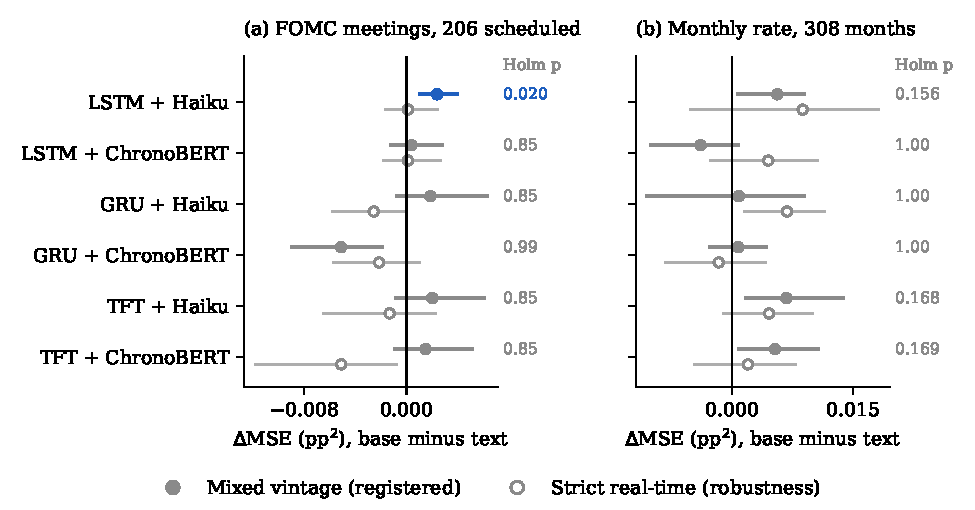
\includegraphics[width=\textwidth]{figures/fig_forest.pdf}
\caption{Gain from adding Fed stance to the networks: $\dmse$ (base minus text, pp$^2$) with 90\% paired
block-bootstrap intervals. Filled markers: registered mixed-vintage comparisons, with Holm-adjusted $p$ on the
right. Hollow markers: the same comparisons with strictly real-time inputs (robustness, outside the Holm family).
Bootstrap intervals are unadjusted.}\label{fig:forest}
\end{figure}

\subsection{Which model forecasts best}

Market prices dominate. The best monthly model is ridge with S+M+N (RMSE 0.1316), nearly tied with S+M (0.1333)
and well ahead of the no-change forecast (0.1813). On meetings, the ordered logit with S+M+N has the highest
accuracy, 90.8\% on the 206 scheduled meetings, while the lowest meeting RMSE (0.122) belongs to the strict-input
GRU without text. These rankings were not tested and are descriptive. The linear models match or beat the networks
at a small fraction of the computational cost.

%======================================================================
\section{Robustness}\label{sec:robust}
%======================================================================

Sections~\ref{sec:cutoff} and~\ref{sec:june} were added after the main results had been seen and are exploratory.

\subsection{Corrected monthly cutoff}\label{sec:cutoff}

Table~\ref{tab:cutoff} reruns the Plan~1 monthly models on the corrected cutoff with all settings unchanged. The
statistics-only model loses information it should not have had, and its RMSE rises from 0.1798 to 0.1919; the
model with text barely moves. The registered test for the headline comparison moves from $p=0.077$ to $0.103$.
The meeting models and networks already used valid cutoffs and are unaffected.

\begin{table}[ht]\centering\footnotesize\setlength{\tabcolsep}{3.5pt}
\begin{threeparttable}
\caption{Plan 1 monthly ridge models on the original and corrected cutoffs}\label{tab:cutoff}
\begin{tabular}{lccccc}
\toprule
& \multicolumn{2}{c}{RMSE (pp)} & $\dmse$ [90\% CI] & \multicolumn{2}{c}{$p$} \\ \cmidrule(lr){2-3}\cmidrule(lr){5-6}
Comparison & Corrected & Original & Corrected & Corrected & Original \\ \midrule
S $\to$ S+N (H1) & 0.1919 $\to$ 0.1675 & 0.1798 $\to$ 0.1664 & $+0.0088$ [$-0.0001$, $+0.0219$] & 0.103 & 0.077 \\
S $\to$ placebo & 0.1919 $\to$ 0.1917 & 0.1798 $\to$ 0.1890 & $+0.0001$ [$-0.0005$, $+0.0012$] & 0.439 & 0.858 \\
No change $\to$ shuffled & 0.1813 $\to$ 0.1824 & 0.1813 $\to$ 0.1823 & $-0.0004$ [$-0.0020$, $+0.0013$] & 0.750 & 0.737 \\
No change $\to$ S+N (H2c) & 0.1813 $\to$ 0.1675 & 0.1813 $\to$ 0.1664 & $+0.0048$ [$-0.0042$, $+0.0107$] & 0.074 & 0.056 \\
S+M $\to$ S+M+N (H2d) & 0.1333 $\to$ 0.1316 & 0.1311 $\to$ 0.1332 & $+0.0004$ [$-0.0011$, $+0.0025$] & 0.251 & 0.695 \\
\bottomrule
\end{tabular}
\begin{tablenotes}\footnotesize
\item 308 test months. RMSE in pp. $p$: one-sided DM-HLN on squared error.
\end{tablenotes}
\end{threeparttable}
\end{table}

\subsection{Strictly real-time inputs}

With only fully vintaged series, the LSTM + Haiku meeting gain falls to $\dmse=+0.0001$ [$-0.0016$, $+0.0024$]
(RMSE 0.1251 to 0.1246, $p=0.461$; hollow markers in Figure~\ref{fig:forest}). The improvement was not
statistically established in the strict-input analysis. A significant result beside a non-significant one does
not by itself show that the two differ, and because the strict and mixed models use different inputs, their RMSE
levels are compared only descriptively. Of the twelve strict comparisons one has a raw $p$ below 0.05, the monthly
GRU + Haiku ($\dmse=+0.0068$ [$+0.0015$, $+0.0115$], $p=0.014$); strict arms lie outside the Holm family.

\subsection{Influence of June 2020}\label{sec:june}

Figure~\ref{fig:cum} plots the running sum of $d_t$ for the monthly S $\to$ S+N comparison. June 2020 alone
supplies 78\% of the total gain. Without that month $\dmse$ falls from $+0.0088$ to $+0.0019$ and RMSE moves only
from 0.1723 to 0.1666; on the original cutoff the share is 67\%. The monthly text gain is therefore mostly a single
forecast at the zero lower bound rather than a steady improvement.

\begin{figure}[ht]\centering
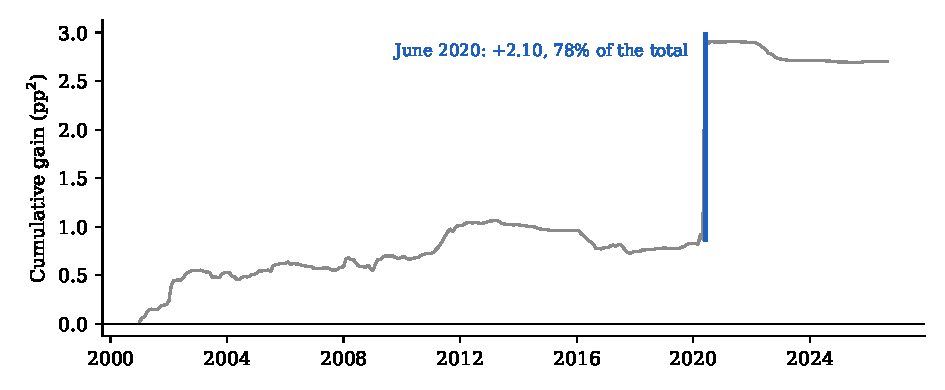
\includegraphics[width=\textwidth]{figures/fig_cumgain.pdf}
\caption{Running sum of the squared-error gain of ridge S+N over ridge S (pp$^2$), corrected monthly cutoff,
308 months. A rising line means text is helping.}\label{fig:cum}
\end{figure}

\subsection{Placebo controls}

No placebo arm improves significantly on its base. In the linear monthly model the placebo moves RMSE from 0.1919
to 0.1917 ($p=0.439$), and the Study~4 Haiku placebo gives $p=0.441$. Across the twelve network placebo arms the
smallest one-sided $p$ against the base model is 0.115. The LSTM + Haiku meeting model also beats its own placebo
($\dmse=+0.0031$ [$+0.0014$, $+0.0046$], $p=0.0008$). Clean placebos argue against spurious structure in the
pipeline, but they cannot detect a reader that recalls outcomes.

\subsection{Interim versus final adjustments}

Two figures circulated in earlier drafts came from incomplete families and are superseded. An adjusted $p$ of
0.014 for LSTM + Haiku was a Holm adjustment over four tests, computed before the TFT arms had finished; over the
registered six it is 0.020. An adjusted McNemar $p$ of 0.045 for the meeting accuracy gain used an interim
family; over the final 15 H2 tests it is 0.146. The code now refuses to report an adjustment until every member of
the registered family is present.

%======================================================================
\section{Discussion and limitations}\label{sec:disc}
%======================================================================

The surviving result is the one most exposed to look-ahead. Haiku's training data run to June 2026, beyond
every test meeting. Asked for decisions by date alone, it recalls 87.8\% of them, and it dates 89.5\% of masked
statements to within one year. A regression of Haiku's gain over ChronoBERT on whether Haiku recalled the decision
finds nothing ($p=0.378$), but only 21 of 211 meetings were not recalled, so that test has little power
\citep[see][on why memorisation evidence is a lower bound]{lopezlira2025}. The LSTM + Haiku gain therefore cannot
be read as skill a forecaster would have had in real time. ChronoBERT, the look-ahead-controlled reader, yields no
gain that survives adjustment.

Further limitations qualify the results.
\begin{itemize}
  \item \textbf{Power.} 308 months and 212 meetings are few for gains of a few percent of RMSE, and errors within
        a policy cycle are correlated. No minimum detectable effect was registered, so a non-significant result
        is not evidence of no effect.
  \item \textbf{Zero lower bound.} About a third of the test window lies at the zero lower bound, where the
        no-change forecast is nearly perfect and a single month can dominate.
  \item \textbf{Revised data.} In the mixed-vintage results 44--45\% of test rows contain a revised statistic.
        These values enter every model identically, but that does not guarantee the bias cancels between models
        with and without text.
  \item \textbf{Hindsight in labels and indices.} The human stance labels were written in 2023--2025, and the
        newspaper-sentiment, geopolitical-risk and policy-uncertainty indices were constructed later with fixed
        methods; their historical revisions could not be verified.
  \item \textbf{Classifier quality.} ChronoBERT is about 64\% accurate on held-out sentences, and the
        sentence-level split makes that figure likely optimistic.
  \item \textbf{Protocol timing.} The network protocol was written after version~1 results were seen. It is
        disclosed and dated, but it is not a pre-registration.
  \item \textbf{Scope.} One country, one target and one stance score per document. Richer representations of
        Fed text were not tested.
\end{itemize}

%======================================================================
\section{Conclusion}\label{sec:concl}
%======================================================================

Fed communication features improved forecasts in some specifications, but the evidence does not yet establish a
consistent and reliable incremental benefit. Text lowers error in most comparisons, yet only one registered test
survives adjustment; that result uses a reader that has seen the test period and is not established with strictly
real-time inputs. Market prices already carry most of what Fed text says about the next decision.

Three extensions would sharpen the answer. A longer or multi-country sample, or live forecasts made after a
reader's training cutoff, would raise power and remove memorisation. Richer measures than a single stance
score---for example the content of forward guidance, or the surprise relative to market expectations---may
capture what a tone index misses. A complete real-time data set for the statistics would remove the remaining
revised values. Until then, the safest reading is that Fed text is a weak and unstable complement to market
prices, not a substitute for them.

\bibliographystyle{plainnat}
\bibliography{refs}

\appendix
\clearpage
%======================================================================
\section{Strict real-time network results}\label{app:strict}
%======================================================================

\begin{table}[ht]\centering\footnotesize\setlength{\tabcolsep}{3.5pt}
\begin{threeparttable}
\caption{Neural networks, strictly real-time inputs (robustness)}\label{tab:strict}
\begin{tabular}{llccccc}
\toprule
Task & Network + reader & Base & + text & $\dmse$ [90\% CI] & NW $p$ & Accuracy (\%) \\ \midrule
T2 & LSTM + Haiku      & 0.1251 & 0.1246 & $+0.0001$ [$-0.0016$, $+0.0024$] & 0.461 & 81.6 $\to$ 85.4 \\
T2 & LSTM + ChronoBERT & 0.1251 & 0.1247 & $+0.0001$ [$-0.0018$, $+0.0026$] & 0.467 & 81.6 $\to$ 84.5 \\
T2 & GRU + Haiku       & 0.1222 & 0.1323 & $-0.0026$ [$-0.0058$, $-0.0001$] & 0.925 & 83.0 $\to$ 86.4 \\
T2 & GRU + ChronoBERT  & 0.1222 & 0.1306 & $-0.0021$ [$-0.0058$, $+0.0010$] & 0.849 & 83.0 $\to$ 85.9 \\
T2 & TFT + Haiku       & 0.1358 & 0.1405 & $-0.0013$ [$-0.0065$, $+0.0023$] & 0.688 & 87.4 $\to$ 87.9 \\
T2 & TFT + ChronoBERT  & 0.1358 & 0.1534 & $-0.0051$ [$-0.0118$, $-0.0007$] & 0.935 & 87.4 $\to$ 86.9 \\ \midrule
T1 & LSTM + Haiku      & 0.1972 & 0.1736 & $+0.0087$ [$-0.0051$, $+0.0182$] & 0.117 & 53.6 $\to$ 58.4 \\
T1 & LSTM + ChronoBERT & 0.1972 & 0.1854 & $+0.0045$ [$-0.0026$, $+0.0106$] & 0.132 & 53.6 $\to$ 55.5 \\
T1 & GRU + Haiku       & 0.1841 & 0.1645 & $+0.0068$ [$+0.0015$, $+0.0115$] & 0.014 & 59.4 $\to$ 63.6 \\
T1 & GRU + ChronoBERT  & 0.1841 & 0.1885 & $-0.0017$ [$-0.0082$, $+0.0042$] & 0.669 & 59.4 $\to$ 59.4 \\
T1 & TFT + Haiku       & 0.1859 & 0.1731 & $+0.0046$ [$-0.0010$, $+0.0100$] & 0.084 & 53.6 $\to$ 56.5 \\
T1 & TFT + ChronoBERT  & 0.1859 & 0.1806 & $+0.0020$ [$-0.0046$, $+0.0079$] & 0.305 & 53.6 $\to$ 50.0 \\
\bottomrule
\end{tabular}
\begin{tablenotes}\footnotesize
\item Base: eight fully vintaged statistics (plus M in T2). Other definitions as in Table~\ref{tab:nets}. Strict
arms are robustness checks and are not Holm-adjusted.
\end{tablenotes}
\end{threeparttable}
\end{table}

%======================================================================
\section{Provenance of results}\label{app:prov}
%======================================================================

\begin{table}[ht]\centering\small
\caption{Where each result comes from}\label{tab:prov}
\begin{tabular}{p{4.6cm}p{3.6cm}p{3.4cm}p{3.2cm}}
\toprule
Result & Code & Commit, date & Status \\ \midrule
Plan 1 linear tests, original cutoff & \texttt{walkforward.py}, \texttt{evaluate.py} & 8c8d3c2, 2026-10-09, after tag \texttt{prereg} & Registered; monthly part superseded \\
Plan 1 monthly rerun, corrected cutoff & \texttt{audit/2026-10-13/ rerun\_plan1\_t1b.py} & 2026-10-13, not yet committed & Post-audit correction, exploratory \\
Study 4 ordered logit & \texttt{haiku\_compare.py} & 7879a70, 2026-10-12; design b4a00fd before the run & Primary of an exploratory study \\
Study 4 networks, version 2 & \texttt{tune.py} & 1a31c73, 2026-10-13; protocol 6048e0d & Amendment written after v1 results \\
Study 4 networks, version 1 & \texttt{tune.py} at 74ab18f & 74ab18f & Superseded, not cited \\
Study 5, three meetings ahead & \texttt{study5.py} & 074d2b9, 2026-10-12; design 85de61f & Primary of an exploratory study \\
\bottomrule
\end{tabular}
\end{table}

\noindent The full audit, with recomputed tables for each vintage treatment, is in
\texttt{audit/2026-10-13/AUDIT.md}; figures are produced by \texttt{paper/make\_figures.py} from the committed
result files.

\end{document}
